\begin{table*}[t]
	\caption{Transductive Imputation AUC with 10\% missing data}
	\centering
	\label{10perc}
\begin{small}
		
		\begin{sc}
		\begin{tabular}{llll}
			\toprule
			Model &                      Accuracy &                          
			Macro-F1 &                Macro-F1  \\
			\midrule
			1&1&1&1\\
			
			\bottomrule
		\end{tabular}
		
	\end{sc}
	\end{small}
\end{table*}

\section{Experiments}

Since there is no other fine-grained chemical entity typing datasets to our knowledge, we evaluate fine-grained chemical entity typing on the CHEMET. The experiments can be reproduced using implementations provided in supplement material.
\subsection{Baseline Methods}
\cheng{It would help to clarify what questions we can answer by comparing the proposed methods with these baselines. It seems to me that these baseline methods do NOT use the same amount of information/resources as the proposed method. If so, the improvement may have come from the fact that we have used additional information/resources, which wasn't used in the baseline methods. This wouldn't be a surprising finding as we are expected to do better with more resources/information. The more interesting question here is: what's the best way of exploiting such information? So if possible, it would be great to include stronger baseline methods that use the SAME amount of extra information. This would help showing the proposed  method is better, not just because it has access to more information/resources, but also because the method can better utilize the extra information than a baseline way of using it (e.g., straightforward combination of existing methods to achieve the goal). Ideally, the baseline methods can be aligned with the most relevant previous work discussed in the related work section. This would help us empirically examine/support the novelty of the work in comparison with previous work from multiple perspectives (e.g., the perspective of tackling the complex name mentions, the perspective of multi-modal attention/embedding, and the connection between local context with molecule structure(?). }
 In the experiment, we compared our method with the following state-of-the-art text classification and fine grained entity typing models,
%(NER) 

\noindent \textbf{SciBERT}. SciBert~\cite{scibert} is a Transformer based language model pretrained on sample of 1.14M papers from Semantic Scholar, in which 82\% are from the broad biomedical domain. A linear layer is applied on the embedding of $[$CLS$]$ for classification.

\noindent \textbf{BioBERT}. Similar to SciBert but pretrained on PubMed abstracts (PubMed) and PubMed Central full-text articles (PMC). Similar to SciBRET, a final linear layer is applied for classification.

\noindent \textbf{Latent Type Representation}. \citet{lin2019attentive} used a hybrid classification method beyond binary relevance to exploit type inter-dependency with latent type representation

\noindent \textbf{Fine-Grained Entity Typing in Hyperbolic Space
} Utilized hyperbolic embeddings. If have time.


%\noindent \textbf{Fine-Grained Entity Typing in Hyperbolic Space}. used Hyperbolic embedding



%\noindent \textbf{Baselines}.
%\noindent \textbf{Implementation}


\subsection{Implementation Detail}

follow Hyspa

<ModelName> was implemented using PyTorch \cite{pytorch} and Huggingface Transformers \cite{huggingface} with SciBERT as text encoder. We left model and training parameters and reproducibility details in the appendix for interested readers. 

\subsection{Result}

\subsection{Ablation Study}
To show the improvement made by each of the submodules in our method, we truncate model in the following way

\begin{itemize}[noitemsep,topsep=0pt]
	
	\item w/o multimodal alignment: FFNN
	\item w/o molecule graph: 
	\item w/o description text: 
\end{itemize}


\subsection{Attention Analysis for Structure-Text Alignment}
By the heatmap visualization

\subsection{Error Analysis}
Here we analyzed the remaining errors and categorize the into different cases  (shown in Figure \ref{error_dist}). We discuss the most common ones below

% \begin{figure*}[ht]
% 	\begin{center}
% 		\centerline{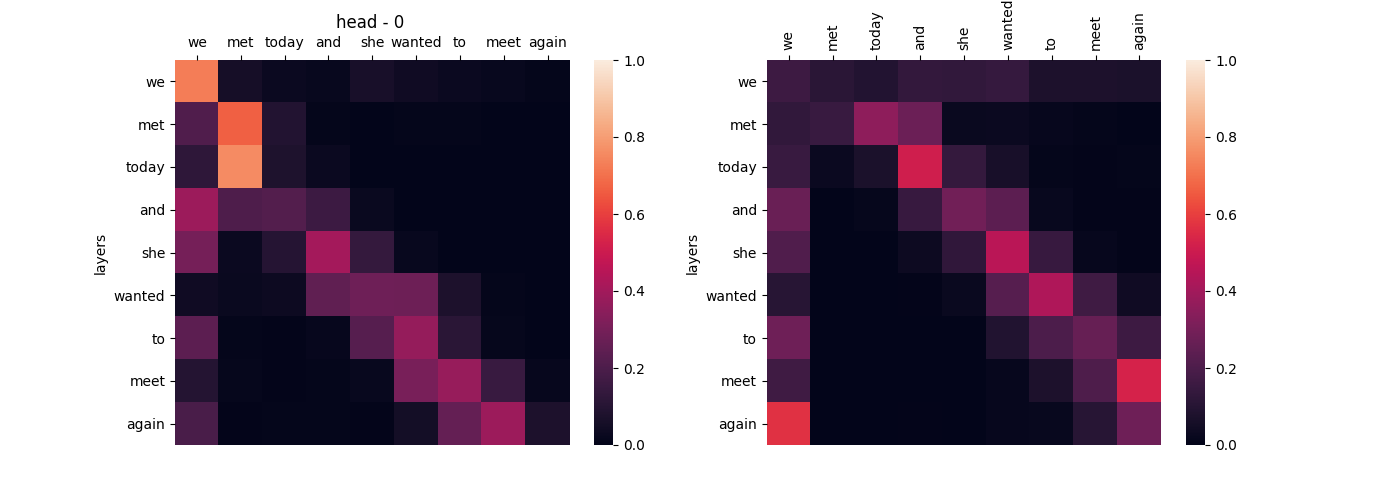
\includegraphics[width=1 
% 			\columnwidth]{attn.png}}
% 		\caption{Self Attention Framework}
% 		\label{fig:attn}
% 	\end{center}
% \end{figure*}

\begin{figure}[t]
	\centering
	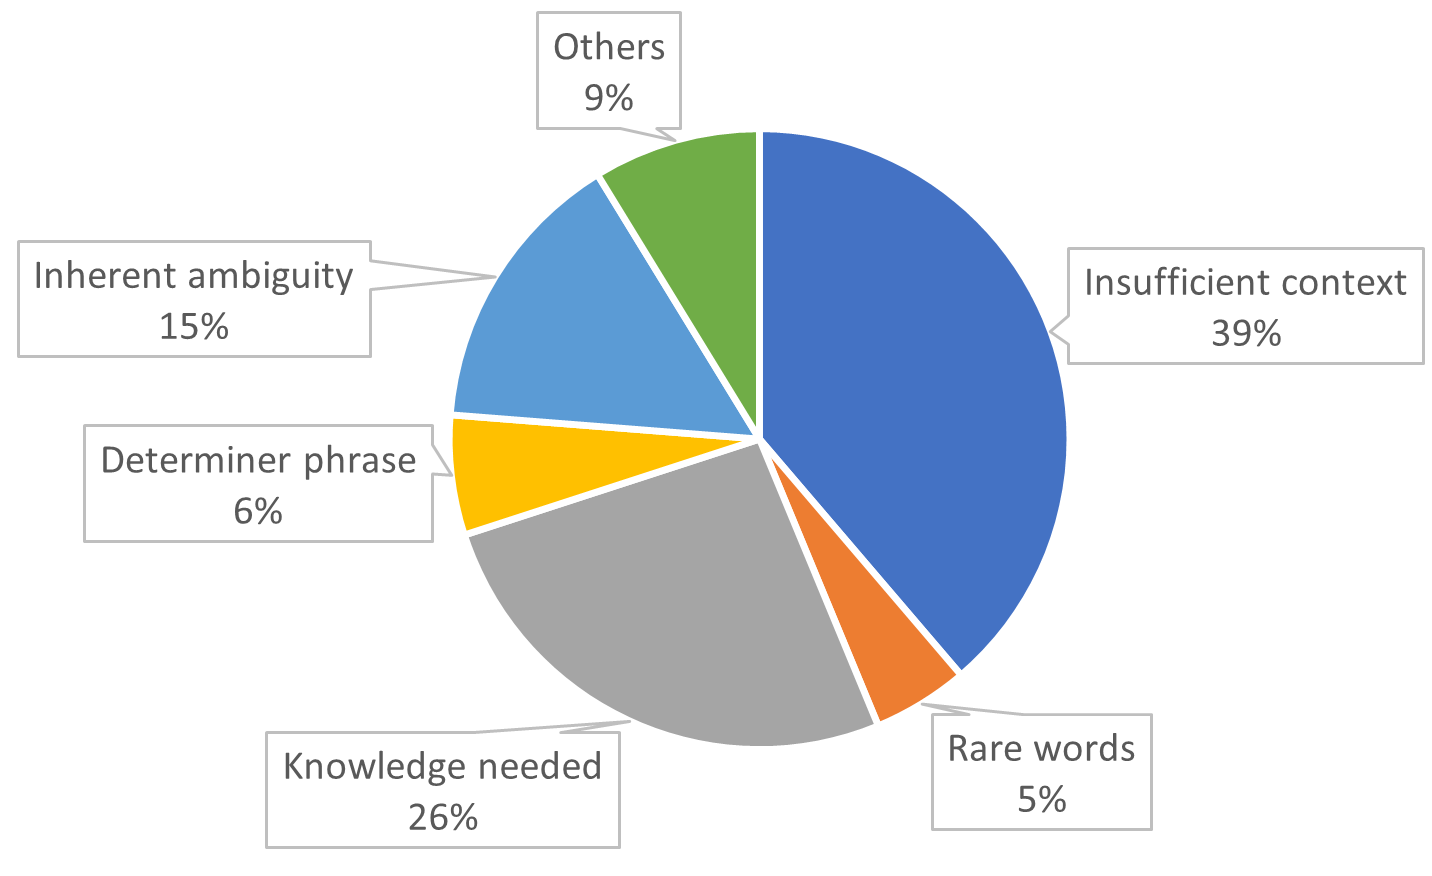
\includegraphics[width=0.9\columnwidth]{case_dist.png}
	\caption{Distribution of remaining errors on the test set.}
	\label{error_dist}
\end{figure}

